\chapter{Theoretical Framework}
\label{sec:framework}
The previous two chapters have given a theoretical overview of the \ac{SM} and
\ac{SUSY}. In order to bring the predictions of these theories closer to the
realm of experiment, this chapter will provide a higher-level discussion more
suited to the results that will be presented later on.

A brief account of vector boson production at a hadron collider is given in
\sec~\ref{sec:framework_wpol}, along with details of the polarisation of \PW
bosons at the \ac{LHC}. This motivates the measurement described in
\chap~\ref{sec:wpol} and forms the framework within which the experimental
results will be interpreted.

In the second part of this chapter, several models relevant to \ac{SUSY}
searches will be presented. These contain a relatively low-dimensional parameter
space, making them convenient for the interpretation of experimental
results. This will be highly relevant to \chap~\ref{sec:interpretation}, where
the models will be applied to the results of the \ac{SUSY} search presented in
\chap~\ref{sec:susysearch}.

\section[W Polarisation]{Polarisation of \PW Bosons}\label{sec:framework_wpol}
Some theoretical background relating to the \ac{SM} has been presented in
\sec~\ref{sec:sm}. Here, theoretical material relating to massive vector boson
production at hadron colliders will be briefly summarised. Then material
relating specifically to the polarisation of \PW bosons will be covered in
detail.

\subsection{Vector Boson Production at Hadron Colliders}
\label{sec:framework_vboson}
A detailed account of massive vector boson production at hadron colliders can be
found in~\cite{nadolsky,pink_book,qcd_primer}. These processes are often
referred to as \Wjets and \Zjets -- meaning production of a \PW or \PZ boson in
association with jets. At hadron colliders, production proceeds predominantly
via $\Pquark\APquark$ or $\Pquark\Pgluon$ interactions and so is strongly
dependent on \ac{QCD} calculations. Cross-sections can be calculated as the
product of the hard scattering cross-section, evaluated in perturbative
\ac{QCD}, with a \ac{PDF}.

The \ac{PDF} is a probability density function giving the probability of finding
a certain parton with a given fraction of the longitudinal momentum, $x$, as a
function of the momentum transfer, $Q^2$. It is obtained from a fit of a
parameterised model to hadronic data. Cross-section calculations for these
processes may be referred to as \acf{LO} or \acf{NLO} This indicates the
precision of the calculation in terms of the expansion of the strong coupling
constant, \alphas~\cite{ellis_wp3jet}.

These processes have been extensively studied and significant recent progress
made, particularly for calculation of higher jet multiplicity
observables~\cite{berger_left_handed_w,berger_nlo_qcd_wjet}. The \Wjets
cross-section has been calculated at \ac{NLO} for up to 4
jets~\cite{berger_wp4jet}. The discussion will now turn to aspects relevant to
\Wjets production and in particular the polarisation effects.

\subsection{Polarisation Effects Parallel to the Beam Line}
For small values of \PW transverse momentum, \PtW, the differential angular
cross-section for the process
$\Pp\Pp\longrightarrow\PWpm\longrightarrow\Plpm\Pgnl$ follows the Drell-Yan
distribution,
\begin{equation*}
\frac{dN}{d(\cos\theta)} \propto (1\mp \cos\theta)^2.
\end{equation*}

It is well known from straightforward helicity arguments~\cite{mirkes_w_1994}
that \PW bosons produced along the beam axis will exhibit a 100\% left-handed
polarisation. This can be seen by considering the leading order partonic
subprocesses,
\begin{equation*}
\Pup\APdown \longrightarrow \PWp \qquad\textrm{and}\qquad
\Pdown\APup\longrightarrow\PWm.
\end{equation*}
Firstly, note that in the case of valence quarks, the fraction of the proton
momentum carried by the quark (as determined by the \aclp{PDF}) is greater than
that of the anti-quark. In addition given that the \ac{LHC} is a $\Pp\Pp$
collider, valence anti-quarks are not present. Anti-quarks must be drawn from
the sea and are therefore likely to be low momentum. Taking these two facts
together, the quark is very likely to have higher momentum than the
anti-quark. By momentum conservation, it is expected that the \PW boson will be
produced overwhelmingly in the direction of the original quark. Then, given the
\VminusA nature of the weak interaction (see \sec~\ref{sec:sm_electroweak}), it
is seen that the quark must be left-handed. Therefore, by helicity conservation,
the \PW will be polarised nearly 100\% left-handedly along the beam axis. A
small dilution will occur in instances where the anti-quark has, by chance, a
larger momentum fraction than the quark.

It is worth mentioning that the situation is not identical at the Tevatron
$\Pp\Pap$ collider. Although the \PWp also possess a 100\% left-handed
polarisation along the beam-line (via similar arguments to those given above),
the \PWm are found to have a near 100\% right-handed polarisation. This is a
result of the subprocess $\APup\Pdown\longrightarrow\PWm$ where this time the
\APup carries more momentum.

% TODO: Mention the effect this has on the rapidity distribution

\subsection{Polarisation Effects in the Transverse Plane}
\label{sec:polarisation}
In the case, where the \PW boson carries a significant transverse momentum, the
situation is more complex. For the sake of this discussion we will consider
cases involving only a single associated jet. Also, in order to simplify
matters, one need only consider the \PWp case, as the \PWm case is very
similar. At leading order, three subprocesses should be
considered~\cite{berger_left_handed_w},
\begin{equation}
\label{eqn:w1jet_processes}
\Pup\Pgluon\longrightarrow\PWp\Pdown\;\textrm{,} \qquad
\Pup\APdown\longrightarrow\PWp\Pgluon\qquad\textrm{and} \qquad
\Pgluon\APdown\longrightarrow\PWp\APup.
\end{equation}
For sufficiently large \PtW, the soft-gluon enhancement of
$\Pup\APdown\longrightarrow\PWp\Pgluon$ is not so significant and the
quark-gluon subprocess is found to dominate. It has been found that 70-80\% of
$\PW+N$~jet ($N \leq 4$) production at \ac{LO} is initiated by this subprocess.

For the quark-gluon subprocess, the $s$ and $t$-channel diagrams are shown in
\fig~\ref{fig:w1jet_st}. For the $s$-channel diagram, the on-shell \Pdown quark
is coupled directly to the \PW and therefore must be in a negative helicity
state (i.e. left-handed). Assuming a positive helicity for the W boson (as
depicted in \fig~\ref{fig:w1jet_st_s}), the spin along the $\PW\Pdown$ axis is
$1+\frac{1}{2} = \frac{3}{2}$. Such a configuration is not allowed for the
\spinhalf off-shell quark and thus the $s$-channel must lead to a 100\%
left-handed polarisation of the \PW.

In contrast, the $t$-channel diagram is not similarly constrained by spin
arguments (since the \PW is not coupled directly to the quark) and thus the
polarisation will not be seen. It can be shown that, for a left-handed incoming
gluon, the $t$-channel diagram can be made to
vanish~\cite{berger_left_handed_w}. Also, for a right-handed gluon, the \PW
polarisation is not constrained, but has been shown to become predominantly
right-handed at high \PtW. The helicity of the outgoing \PW will be almost 100\%
correlated with that of the incoming gluon at high \PtW.

Overall, due to a factor 4 difference in the size of the corresponding matrix
elements, the \PW is expected to asymptotically approach an 80\% left-handed
polarisation at large \PtW. The \VminusA coupling allows the decay leptons to be
used as an analyser of the \PW polarisation. This allows the effect to be
measured. Having given an overview of the physics underlying this effect, a more
detailed argument will now be presented.

\begin{figure}
\centering
\subfloat[]{\label{fig:w1jet_st_s}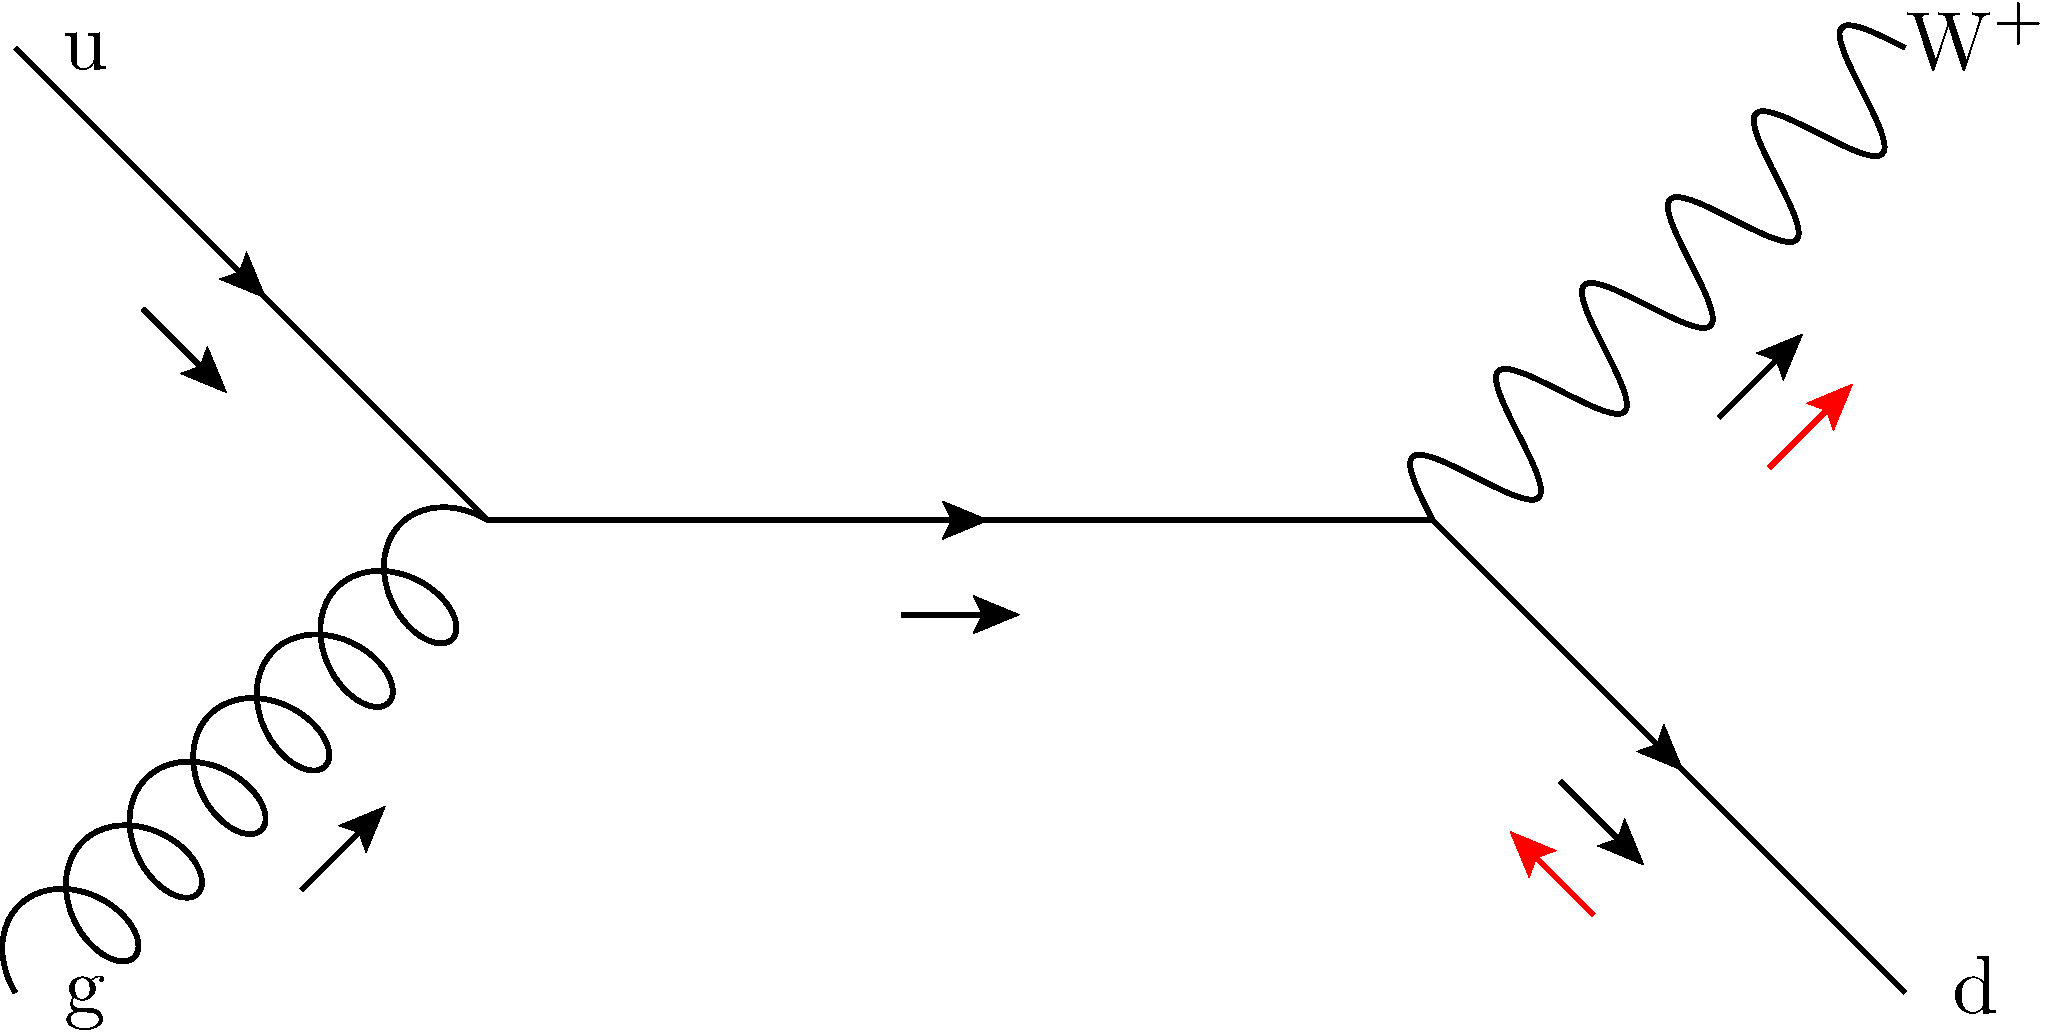
\includegraphics[width=0.5\textwidth]{fig/wpol_1jet_s}}\quad
\subfloat[]{\label{fig:w1jet_st_t}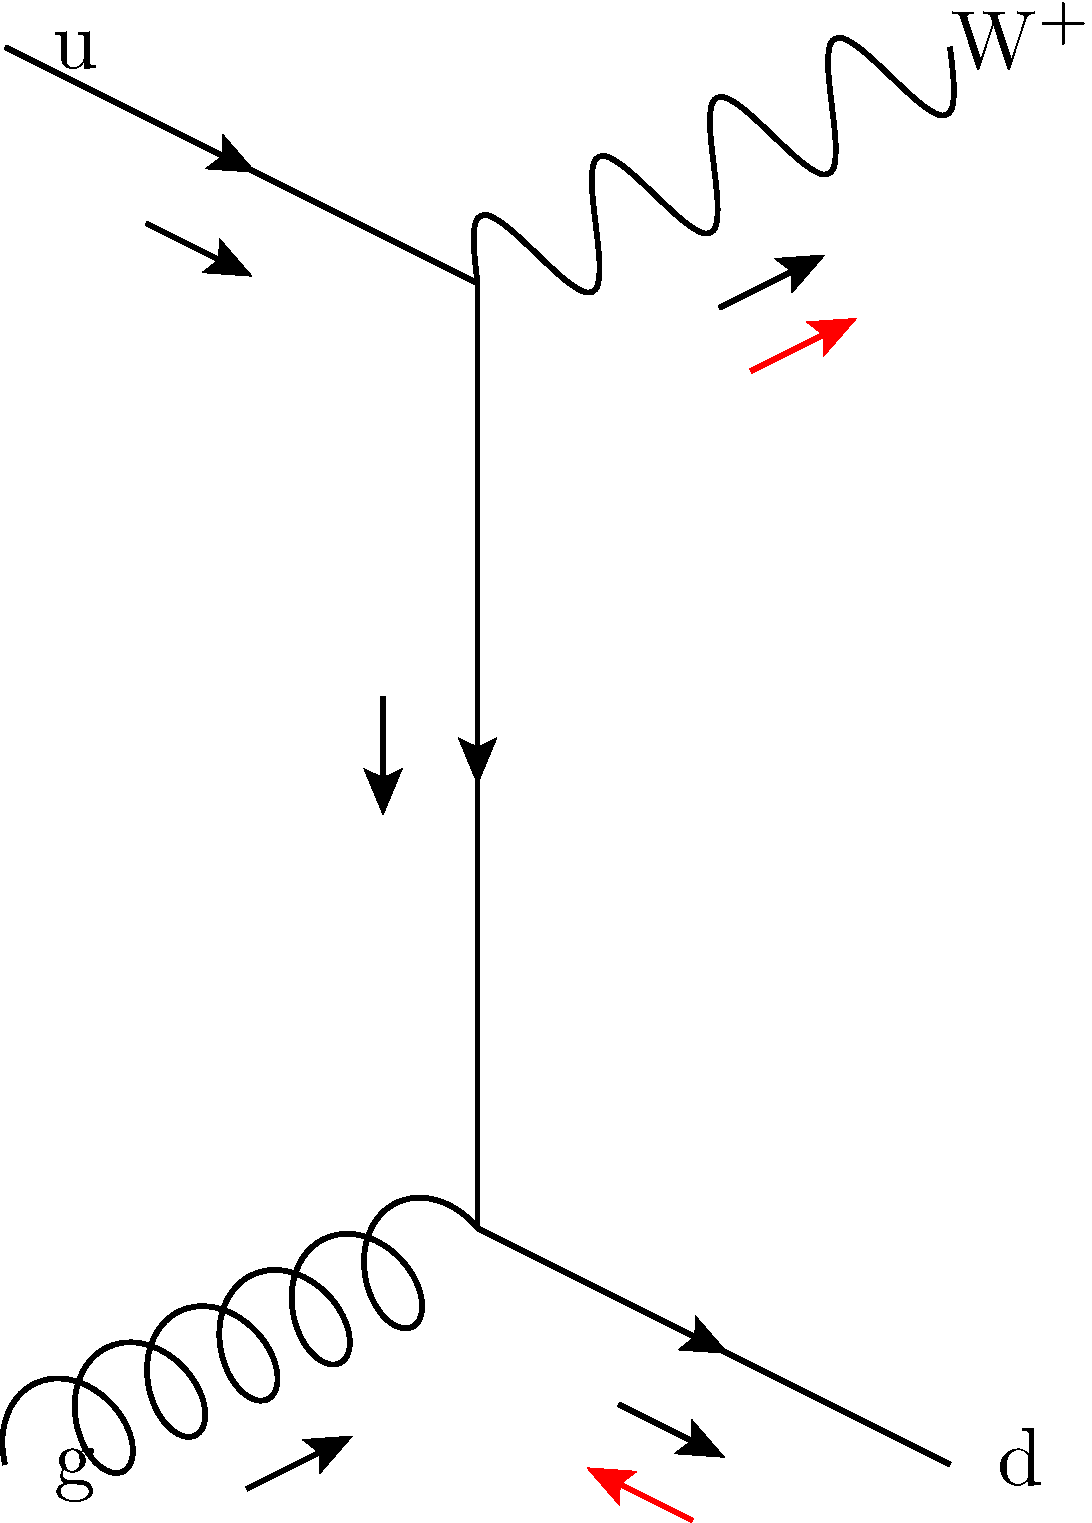
\includegraphics[width=0.25\textwidth]{fig/wpol_1jet_t}}
\caption[Diagrams showing the $\Pup\Pgluon\longrightarrow\PWp\Pdown$
subprocess]{Diagrams showing the $\Pup\Pgluon\longrightarrow\PWp\Pdown$
  subprocess in the \subref{fig:w1jet_st_s} $s$ and \subref{fig:w1jet_st_t} $t$
  channels. The black displaced arrows indicate the particle momenta. The red
  arrows indicate helicity in the case of a right-handed \PW boson and a
  left-handed \Pdown quark.}
\label{fig:w1jet_st}
\end{figure}

Writing the amplitudes of the subprocesses in \eqn~\ref{eqn:w1jet_processes}
in terms of spinor products, two distinct expressions emerge,

\begin{eqnarray*}
\mathcal{A}^{\textrm{tree}}_{(a)} &\propto&
\frac{\left<\Pdown\nu\right>^2}{\left<\Pup\Pgluon\right>\left<\Pgluon\Pdown\right>}\quad\textrm{and}\\
\mathcal{A}^{\textrm{tree}}_{(b)} &\propto&
\frac{\left[\Pup\Pe\right]^2}{\left[\Pup\Pgluon\right]\left[\Pgluon\Pdown\right]},
\end{eqnarray*}
where factors common to both expressions are not shown. The corresponding
cross-sections are
\begin{equation}
\label{eqn:w1jet_xs}
d\sigma^{\textrm{LO}}_{(a)} \propto (k_{\Pdown} \dot k_{\Pneutrino})^2 \quad \textrm{and} \quad
d\sigma^{\textrm{LO}}_{(b)} \propto (k_{\Pup} \dot k_{\Pe})^2,
\end{equation}
where the $k$ are Lorentz vectors representing the particle momenta. For each
subprocess, the helicity configurations corresponding to $(a)$ and $(b)$ are
shown in the upper and lower rows of \fig~\ref{fig:w1jet_modes}
respectively. The red arrows indicate particle helicity, with a double-stemmed
arrow for the \PW momentum. In the cases where the \PW boson is neither purely
left-handed nor right-handed, the arrow is placed at an angle.

Starting with the subprocess $\Pup\Pgluon\longrightarrow\PWp\Pdown$, the $(a)$
expression in \ref{eqn:w1jet_xs} correlates the axis of the \Pdown quark with
the neutrino. This is shown in \fig~\ref{fig:w1jet_modes_1a}. The \VminusA
coupling requires the neutrino to have a left-handed helicity. By angular
momentum conservation, the \PW boson must also be left-handed. The angular
dependence is $(1-\cos\tilde{\theta}^*)^2$ where $\tilde{\theta^*}$ is the angle
of the charged decay lepton with respect to the \PW flight direction in the
centre-of-mass frame. In contrast, consider an identical particle configuration,
but with helicities corresponding to $(b)$. This is shown in
\fig~\ref{fig:w1jet_modes_1b}. The \Ppositron direction is now correlated with
the incoming beam direction. Boosting to the \PW rest frame, at high \PtW, the
incoming quark and gluon are nearly parallel. Thus, given a scattering angle of
90\degrees, the \Pup quark momentum is seen to be half that of the \Pdown
quark. The angular dependence is thus $\frac{1}{4}(1+\cos\tilde{\theta}^*)^2$,
yielding a right-handed polarisation at a quarter of the rate of the left-handed
component.

For the sub-dominant process $\Pup\APdown\longrightarrow\PWp\Pgluon$, the terms
in \eqn~\ref{eqn:w1jet_xs} correlate the momenta of the decay leptons with the
beam direction. The two cases are shown in \figs~\ref{fig:w1jet_modes_2a} and
\ref{fig:w1jet_modes_2b}. Although it can be seen once again that a left-handed
and right-handed polarisation emerge, in this case they are found to cancel for
a scattering angle of 90\degrees and thus give no net polarisation
effect. Lastly, for the subprocess $\Pgluon\APdown\longrightarrow\PWp\APup$,
shown in \figs~\ref{fig:w1jet_modes_3a} and \ref{fig:w1jet_modes_3b}, the $(b)$
contribution correlates the \Pup quark and the \Ppositron direction, leading to
a dominantly right-handed polarisation. However, since the \ac{PDF},
$\APdown(x)$, is much smaller than $\Pup(x)$, this effect is largely washed out
by the dominant left-handed polarisation mode.

\begin{figure}
\centering
\subfloat[]{\label{fig:w1jet_modes_1a}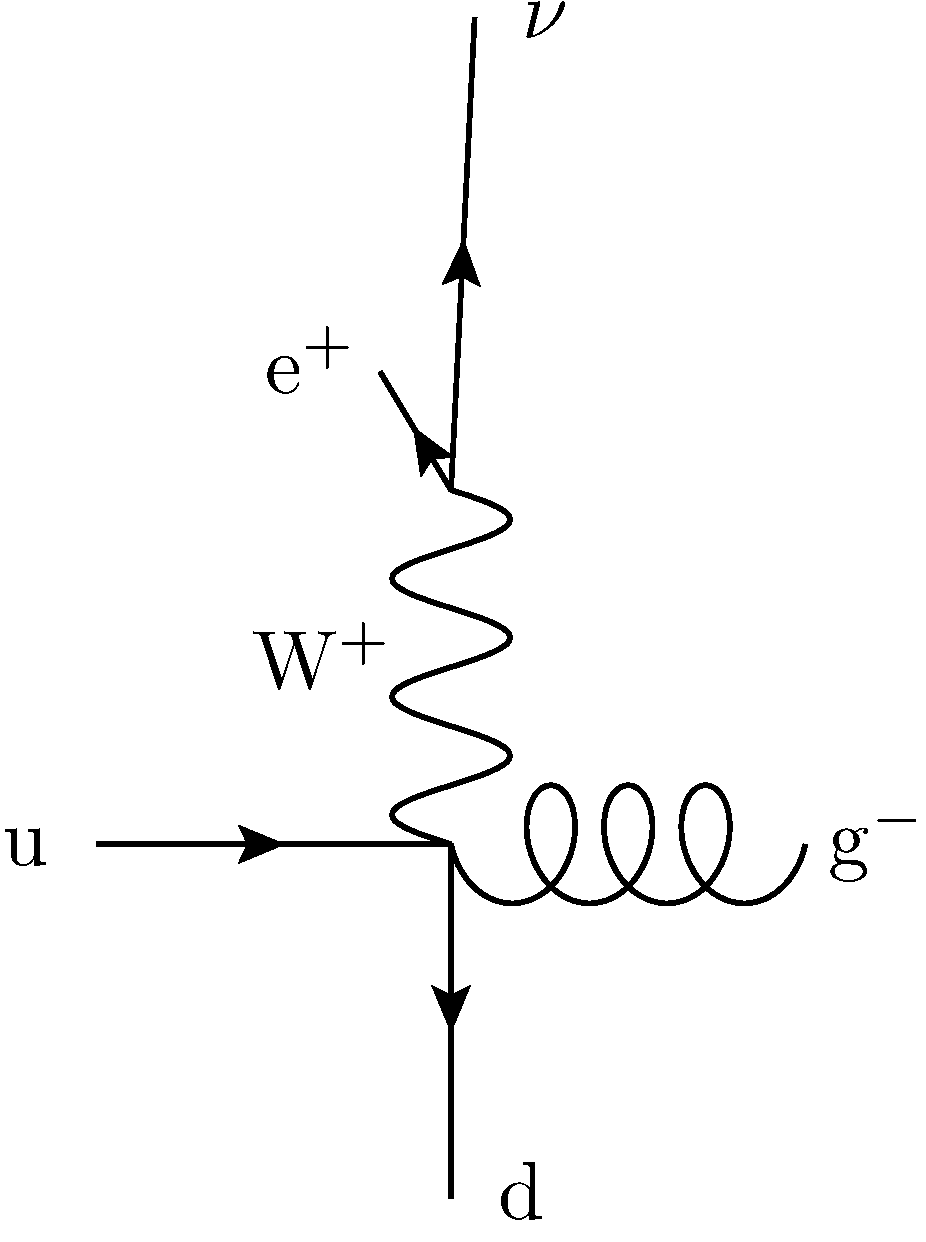
\includegraphics[width=0.27\textwidth]{fig/wpol_prod_a}}\quad
\subfloat[]{\label{fig:w1jet_modes_2a}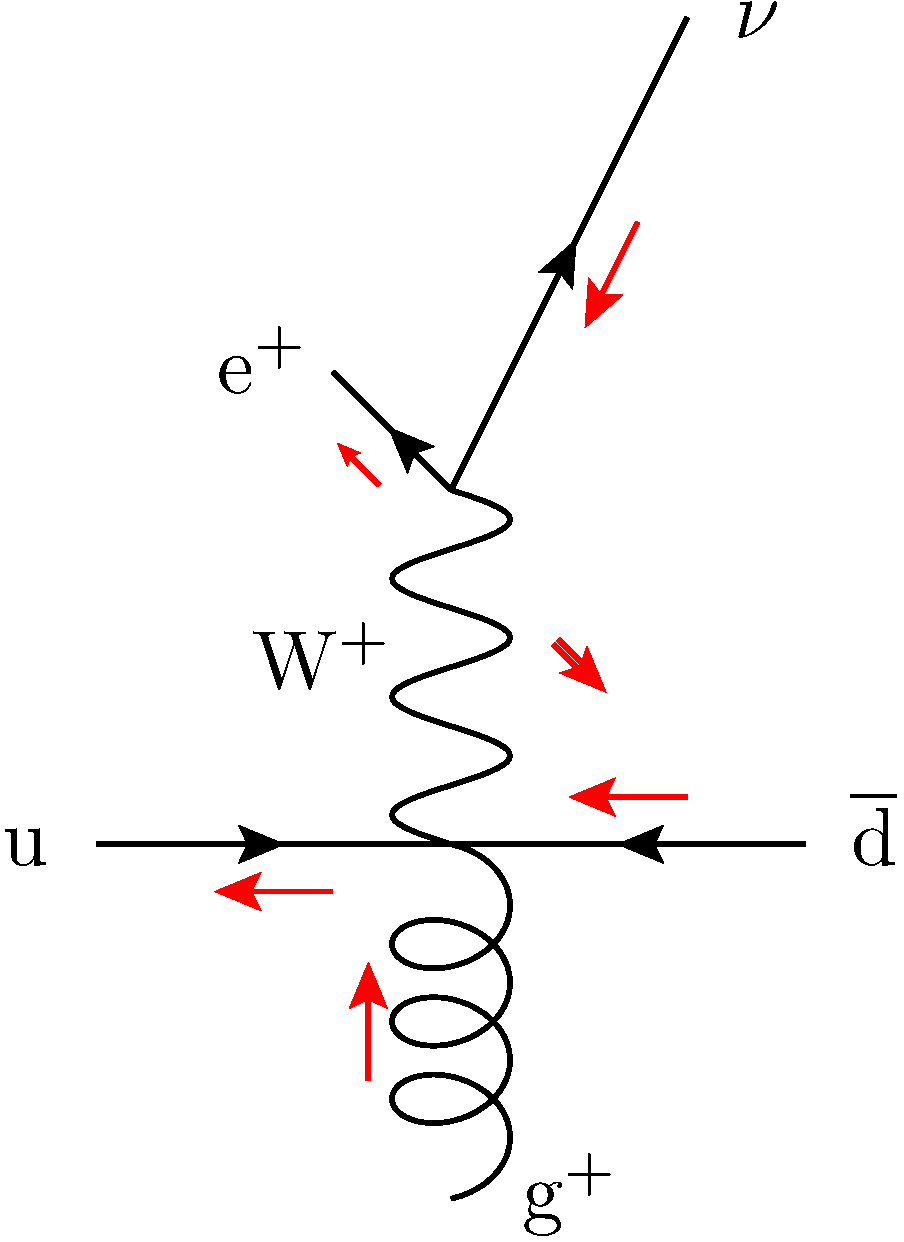
\includegraphics[width=0.27\textwidth]{fig/wpol_prod_b}}\quad
\subfloat[]{\label{fig:w1jet_modes_3a}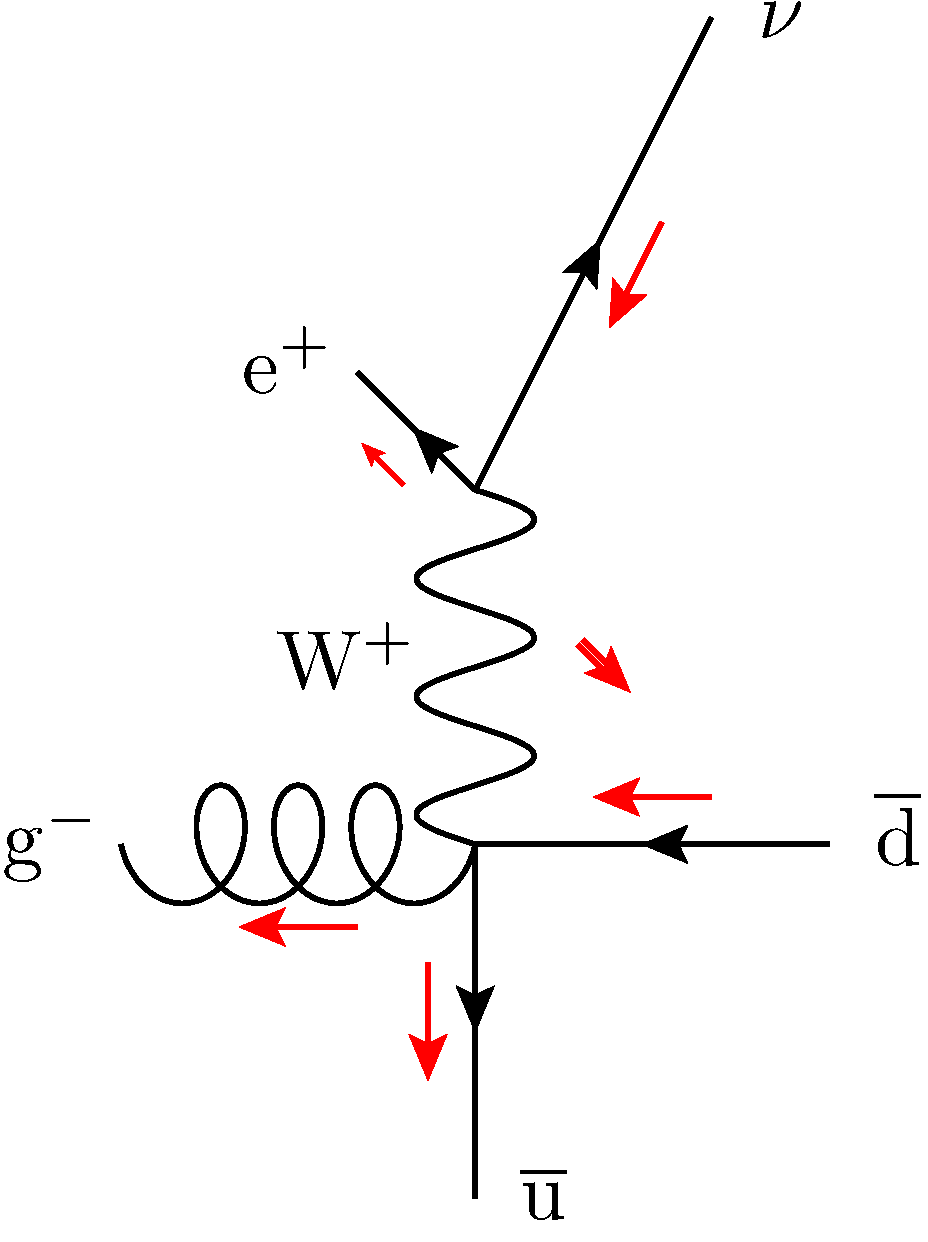
\includegraphics[width=0.27\textwidth]{fig/wpol_prod_c}}\\
\subfloat[]{\label{fig:w1jet_modes_1b}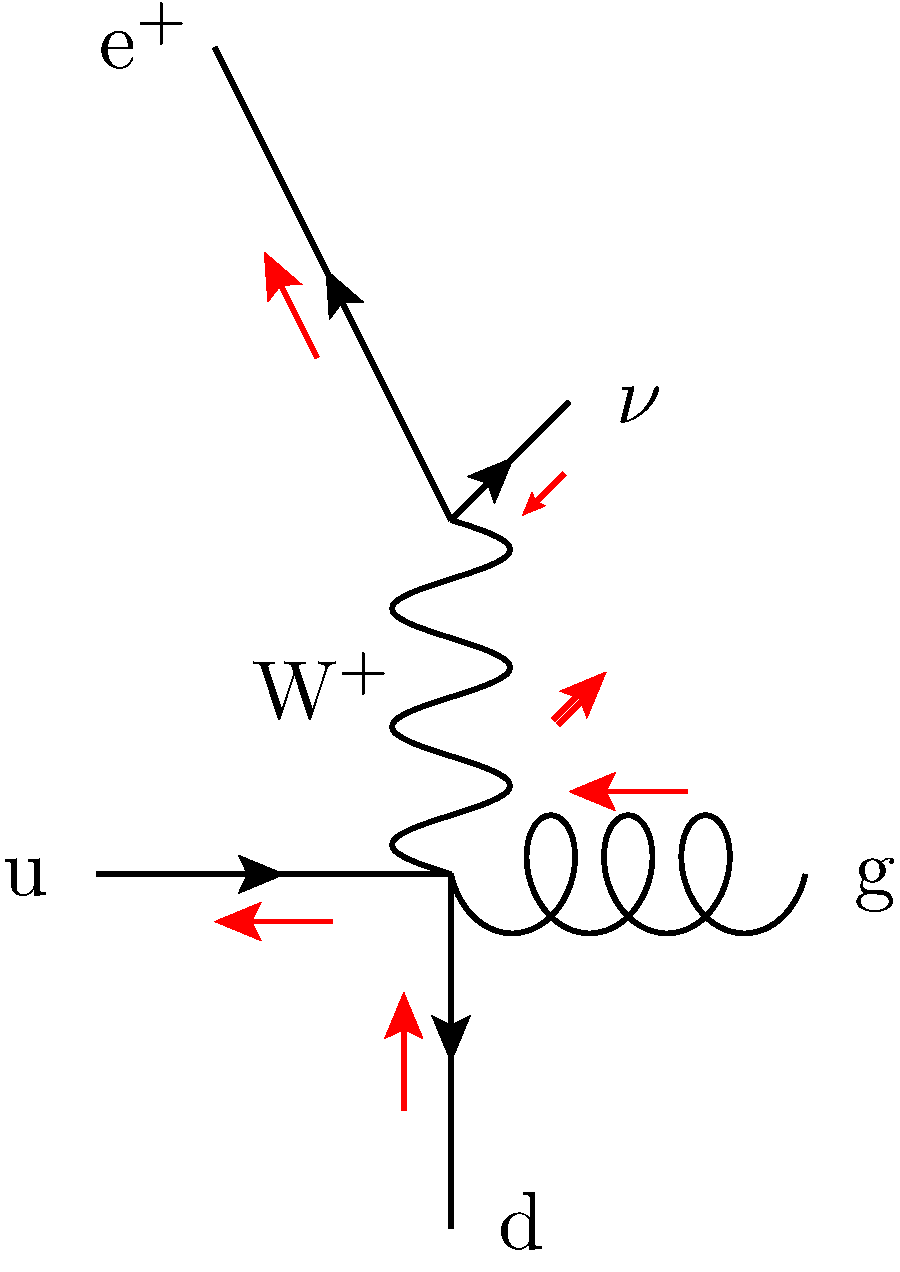
\includegraphics[width=0.27\textwidth]{fig/wpol_prod_d}}\quad
\subfloat[]{\label{fig:w1jet_modes_2b}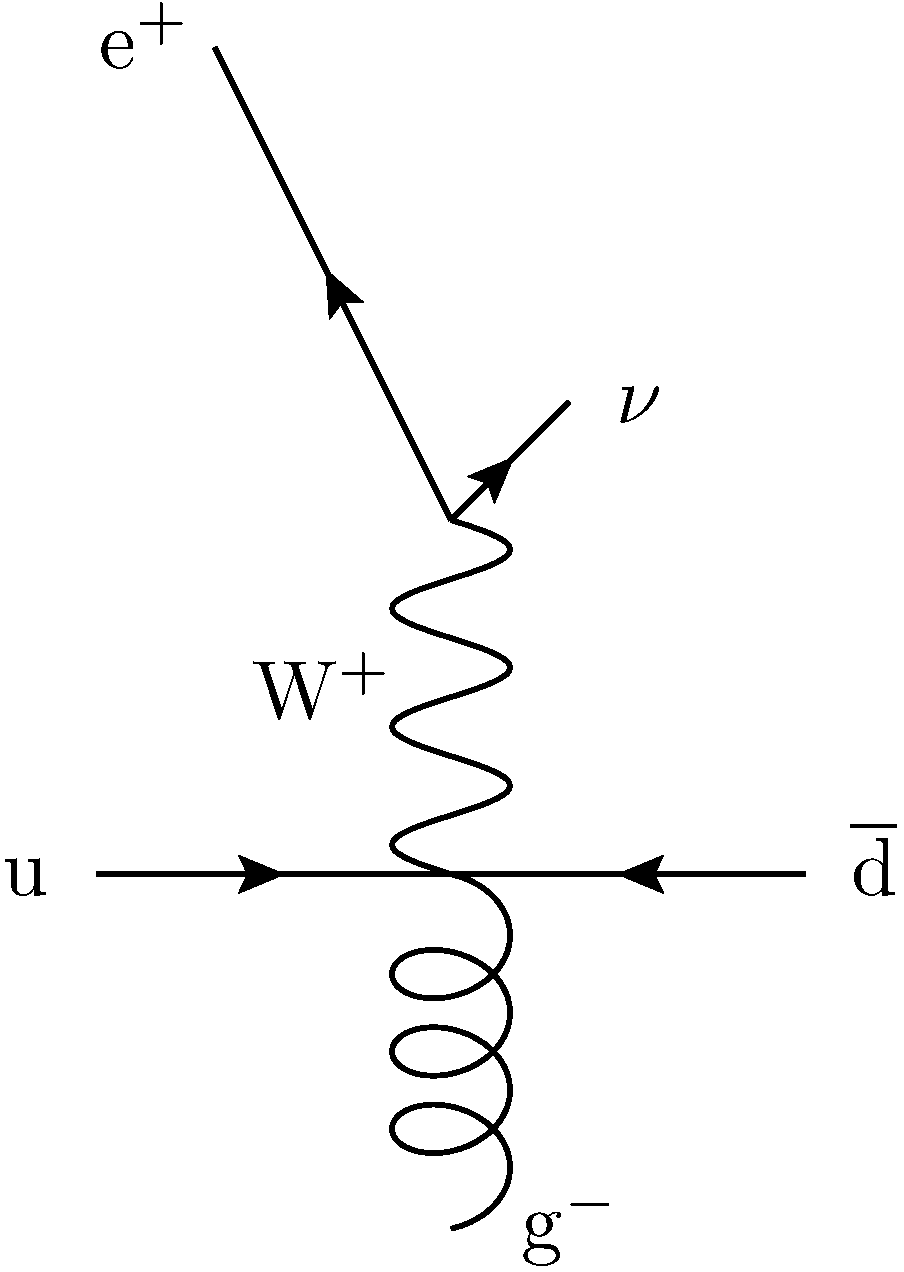
\includegraphics[width=0.27\textwidth]{fig/wpol_prod_e}}\quad
\subfloat[]{\label{fig:w1jet_modes_3b}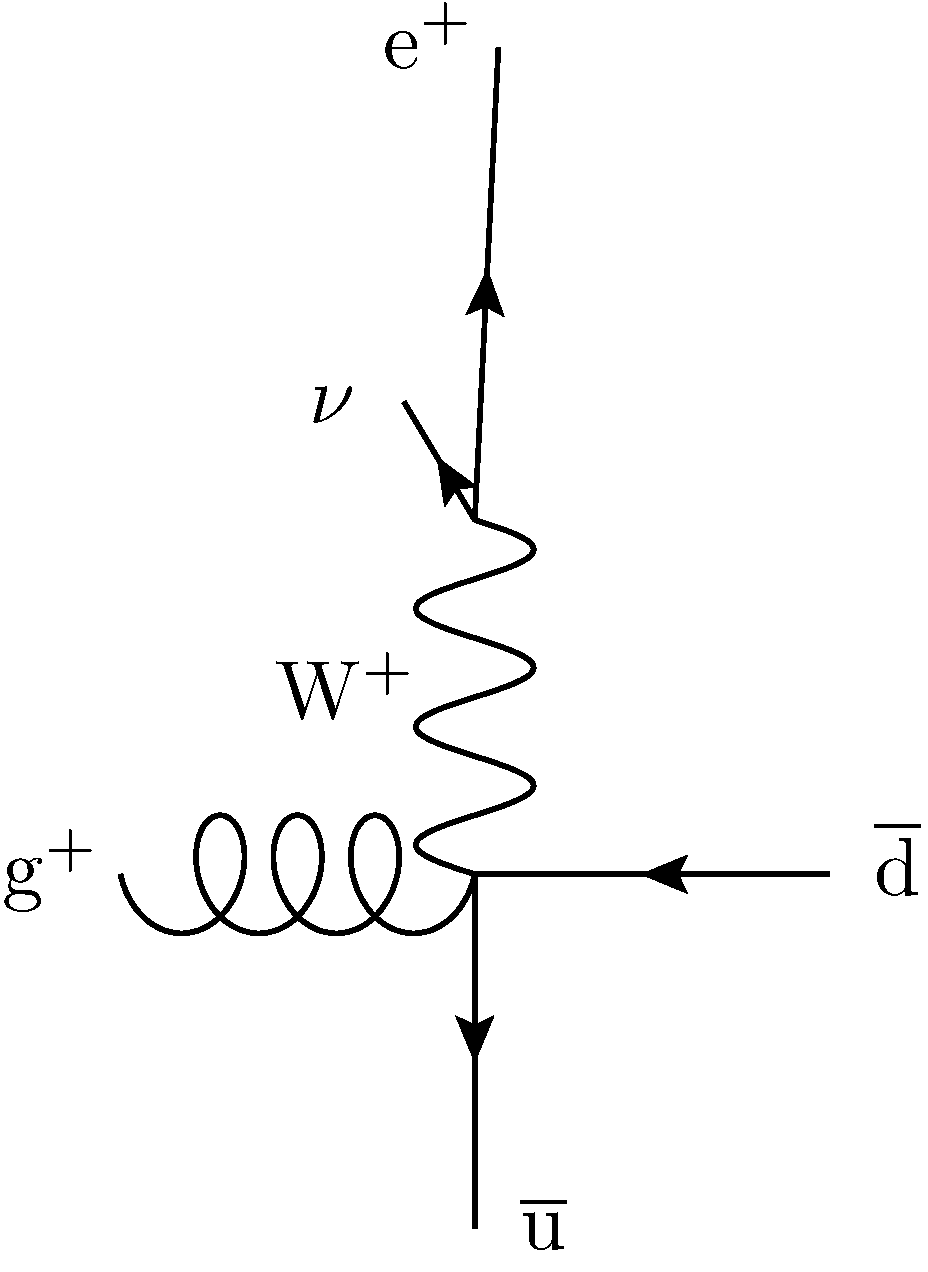
\includegraphics[width=0.27\textwidth]{fig/wpol_prod_f}}
\caption[Illustrations of $\PWplus+1$~jet production modes at the
LHC]{Illustrations of $\PWplus+1$~jet production modes at the LHC. Red
  single-stemmed arrows represent particle helicity. Red double-stemmed arrows
  indicate the polarisation of the \PW boson. In cases where the \PW is not
  produced with a definite polarisation, the arrow is placed at an angle. The
  angles and sizes of the particle lines are suggestive of their momenta in the
  centre-of-mass frame.}
\label{fig:w1jet_modes}
\end{figure}

It has been seen that the proton-proton environment at the \ac{LHC} is expected
to lead to a dominance of left-handed over right-handed helicity states for \PW
bosons with large transverse momentum. In order to observe this effect, the
helicity of \PW bosons must be measured. This will be discussed in the next section.

\subsection{Measuring Helicity}
\subsubsection{The Helicity Frame}
Polarisation effects may be conveniently studied within the helicity frame of
the \PW boson. This is illustrated in \fig~\ref{fig:wpol_helicity_frame}. The
helicity frame is defined in the rest frame of the \PW boson, with the
polarisation axis (here, the z-axis) aligned along the \PW line-of-flight in the
lab frame. The x-axis is then chosen to lie along the plane spanned by the two
colliding protons in the boson rest frame. The sense is chosen such that the
angle between the axis and the nearest proton is minimised. The y-axis is then
fixed to be perpendicular to these two (the coordinate system is
right-handed). The polar angle, \thetastar is measured in the $y-z$ plane
between the positive z-axis and the lepton. Likewise, the azimuthal angle,
\phistar is measured in the $x-z$ plane, between the positive $x$ axis and the
lepton. For $0 < |\phistar| < \frac{\pi}{2}$, the charged lepton will have a
larger rapidity that the \PW boson and thus a smaller \Pt. Alternatively, for
$\frac{\pi}{2} < |\phistar| < \pi$, the lepton will have a smaller rapidity and
a larger \Pt.

\begin{figure}[htbp!]
%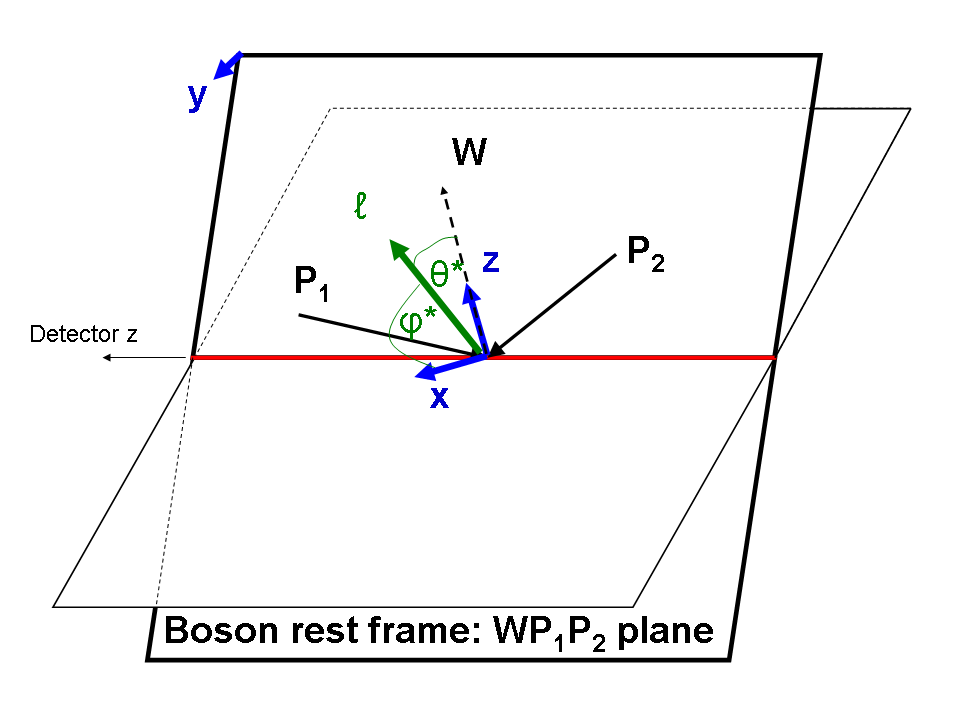
\includegraphics[width=0.8\textwidth]{fig/helicity_frame_polnote}
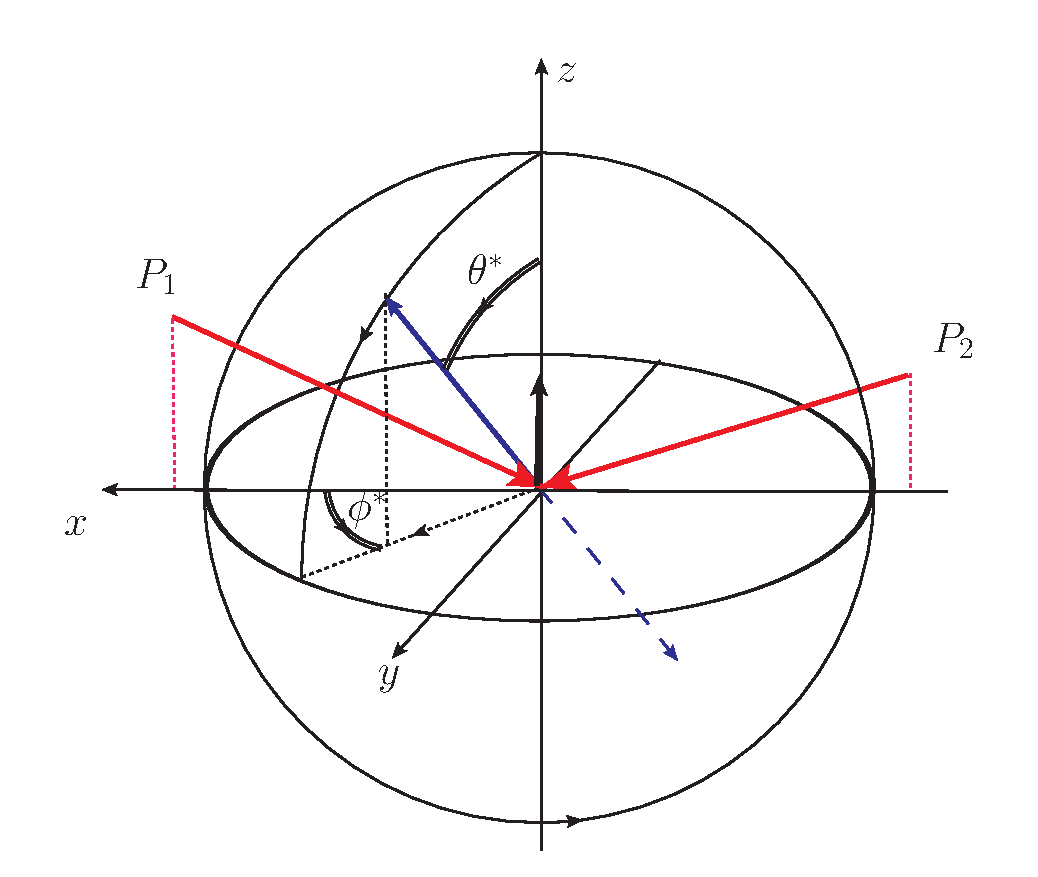
\includegraphics[width=0.6\textwidth]{fig/helicity_frame_better}
\caption[Illustration of the helicity frame]{Illustration of the helicity
  frame~\cite{berger_left_handed_w}. The lines $P_1$ and $P_2$ represent the
  incoming protons boosted into the helicity frame. The blue line indicates the
  direction of the decay lepton. The azimuthal and polar angles, \phistar and
  \thetastar, are also shown.}
\label{fig:wpol_helicity_frame}
\end{figure}

\subsubsection{Quantifying Helicity}
\label{sec:quant_helicity}
The hadronic cross-section of the \PW is obtained within the parton model by
weighting the individual parton-level cross-sections with the respective
\acp{PDF}~\cite{mirkes_w_1994},
\begin{equation*}
\frac{d\sigma^{h_1 h_2}}{d(\PtW)^2 dy d\Omega^*} = \sum_{ab} \int dx_1 dx_2
f_a^{h_1}\left(x_1, \mu_F^2\right)f_b^{h_2}\left(x_2, \mu_F^2\right)
\times \frac{s d\tilde{\sigma}_{ab}}{dt du d\Omega^*} \left(x_1 P_1, x_2 P_2,
\alpha_s (\mu_R^2)\right),
\end{equation*}
where $h_1$ and $h_2$ are the interacting hadrons and the sum runs over $a,b =
\Pquark, \APquark, \Pgluon$. The \acp{PDF}, $f_a^{h}\left(x, \mu^2\right)$, give
the probability of finding a parton $a$ with momentum fraction $x$ in hadron $h$
when probed at a scale $\mu^2$. The $d\tilde{\sigma}_{ab}$ are the parton-level
cross-sections for the chosen process(es). The hadron-level Mandelstam variables
are written in uppercase,
\begin{equation*}
S = (P_1 + P_2)^2 \qquad T = (P_1 - Q)^2 \qquad U = (P_2 - Q)^2,
\end{equation*}
and parton-level in lowercase,
\begin{eqnarray*}
s &=& (p_1 + p_2)^2 = x_1 x_2 S\\
t &=& (p_1 - Q)^2  = x_1(T-Q)^2 +Q^2\\
u &=& (p_2 - Q)^2 = x_2(U -Q)^2 + Q^2,
\end{eqnarray*}
where
\begin{equation*}
p_1 = x_1 P_1 \qquad p_2 = x_2 P_2.
\end{equation*}
The momenta of the incoming hadrons are labelled $P_1$ and $P_2$ and the
interacting partons, $p_1$ and $p_2$. This expression can be rewritten in terms
of a standard set of angular coefficient $A_i$, to give~\cite{mirkes_w_1992}
\begin{align}
\label{eqn:wpol_diff_xs}
\frac{d\sigma}{d(\PtW)^2 dy d\cos\theta d\phi} = \frac{3}{16\pi}
\frac{d\sigma^{-1}}{d(\PtW)^2 dy} &\left [ \left(1+\cos^2\theta\right) \right. \nonumber\\
 &+ \frac{1}{2} A_0 \left ( 1 - 3\cos^2\theta \right ) + A_1 \sin 2\theta\cos\phi \nonumber\\
 &+ \frac{1}{2}A_2\sin^2\theta\cos 2\phi + A_3\sin\theta\cos\phi \nonumber\\
 &+ A_4\cos\theta + A_5\sin^2\theta\sin 2\phi \nonumber\\
 &+ A_6\sin 2\theta\sin \phi + A_7\sin\theta\sin\phi
\end{align}

% TODO: Figure out the difference between  theta and theta*
The $A_i$ are ratios of the separate helicity cross-sections of the boson to its
total unpolarised cross-section. They are dependent on the \PW boson charge,
transverse momentum, \PtW, and rapidity, \YW. \eqn~\ref{eqn:wpol_diff_xs} can be
integrated over $\phi$ and \PtW to give
\begin{equation}
\label{eqn:wpol_xs_Ai}
\frac{d\sigma}{d\cos\theta} \propto \left(1+\cos^2\theta\right) +
\frac{1}{2}A_0\left(1-3\cos^2\theta\right) + A_4\cos\theta.
\end{equation}

% TODO: Check all this bs!
Again, because of the \VminusA coupling, the \PWp (\PWm) may couple only to
left-handed (right-handed) fermions and right-handed (left-handed)
anti-fermions. Therefore the angular momentum state of the decay leptons is
\begin{eqnarray*}
\ket{\Pl\Pgn^{J,M}} &=& \ket{\frac{1}{2}, \pm \frac{1}{2}}
\oplus \ket{\frac{1}{2}, \pm\frac{1}{2}} \\
&=& \textrm{either}\quad\ket{1, +1}\quad\textrm{or}\quad \ket{1, -1},
\end{eqnarray*}
where $\ket{J, M}$ represents an angular momentum state with a total angular
momentum, $J$, and projection, $M$. Rotating these states through the angle
\thetastar, one obtains
\begin{equation}
\ket{\Pl\Pgn^{J,M}}' = \sum_{M'=-J}^{M'=+J} d_{M, M'}^J \ket{J, M'}.
\end{equation}
The angular momentum of a \PW boson in a helicity eigenstate is then
$\ket{\PW^{J,M''}}$. The matrix element for the angular momentum coupling can be
written
\begin{eqnarray*}
\braket{\PW^{J,M''}}{\Pl\Pgn^{J,M}}' &\sim& \sum_{M'=-J}^{M'=+J} d_{M M'}^{J}
\braket{J,M''}{J,M'} \\
&\sim& d^{J}_{M M''} \braket{J,M''}{J,M''} \sim d_{M M''}^{J}.
\end{eqnarray*}
The cross-section is calculated by squaring the matrix elements and summing over
the helicity states ($M''$) of the incoming $\PW$ boson. Each state is weighted
by the helicity fraction $f_{M''}$,
\begin{equation*}
  \sigma(\PW\longrightarrow\Pl\Pgnl) \sim f_0 \left|d_{M 0}^1\right|^2 + f_{-1} \left|d_{M
      -1}^1\right|^2 + f_{1} \left|d_{M +1}^1\right|^2,
\end{equation*}
where $f_0 + f_1 + f_{-1} = 1$. Finally, using the fact that for \PWpm,
$M=\pm1$, and replacing for the elements of the D-matrices in terms of
$\cos\thetastar$ gives,
\begin{equation}
\label{eqn:wpol_helicity_fractions}
\sigma(\thetastar_{\Plpm}) = \frac{\f0}{2}\sin^2\thetastar_{\Plpm} +
\frac{\fL}{4} \left(1\mp\cos\thetastar_{\Plpm}\right)^2 +
\frac{\fR}{4} \left(1\pm\cos\thetastar_{\Plpm}\right)^2.
\end{equation}
Note that the helicity fractions \ffi have been relabelled to give a more
intuitive interpretation as the left-handed, right-handed and longitudinal
polarisation fractions. Comparing now to \eqn~\ref{eqn:wpol_xs_Ai}, we identify
\begin{eqnarray*}
A_0 \sim f_0 \quad\textrm{and}\\
A_4 \sim \pm \fLmfR.
\end{eqnarray*}
Whilst the $A_i$ are the more fundamental parameters from a theoretical point of
view, the helicity fractions \f0, \fL and \fR will often be more convenient for
experimental discussion. The other \Ai parameters will not be discussed in
detail, though their small effect on the measurement of $A_0$ and $A_4$ will be
evaluated.

In \chap~\ref{sec:wpol}, the measurement of the helicity fractions \fL, \fR and
\f0 will be described. The intention of this analysis is to confirm the
prediction that the left-handed mode dominates at high \PtW, or equivalently,
$\fLmfR > 0$. In addition, it is expected that $\fL > \f0$.

The evolution of the polarisation fractions with \PtW has also been studied in
simulation~\cite{berger_left_handed_w}. The evolution of \fL, \fR and \f0 is
shown in \fig~\ref{fig:framework_ptw} for the \PWp case. The increase of \fLmfR
with \PtW can be readily seen. Also, because of the equivalence
theorem~\cite{equiv_theorem,tev_physics,gounaris,cornwall,elementary_pp}, the
behaviour of the longitudinal polarisation mode approximates the corresponding
Goldstone boson (see \sec~\ref{sec:sm_goldstone}) at large \PtW. This explains
the decrease of \f0 as \PtW becomes large.

Whilst the dependence of the polarisation on \PtW make for a very interesting
measurement, it was found to be infeasible with the relatively small data sample
available for this analysis.

\begin{figure}
\centering
\subfloat[\fL]{\label{fig:framework_ptw_fL}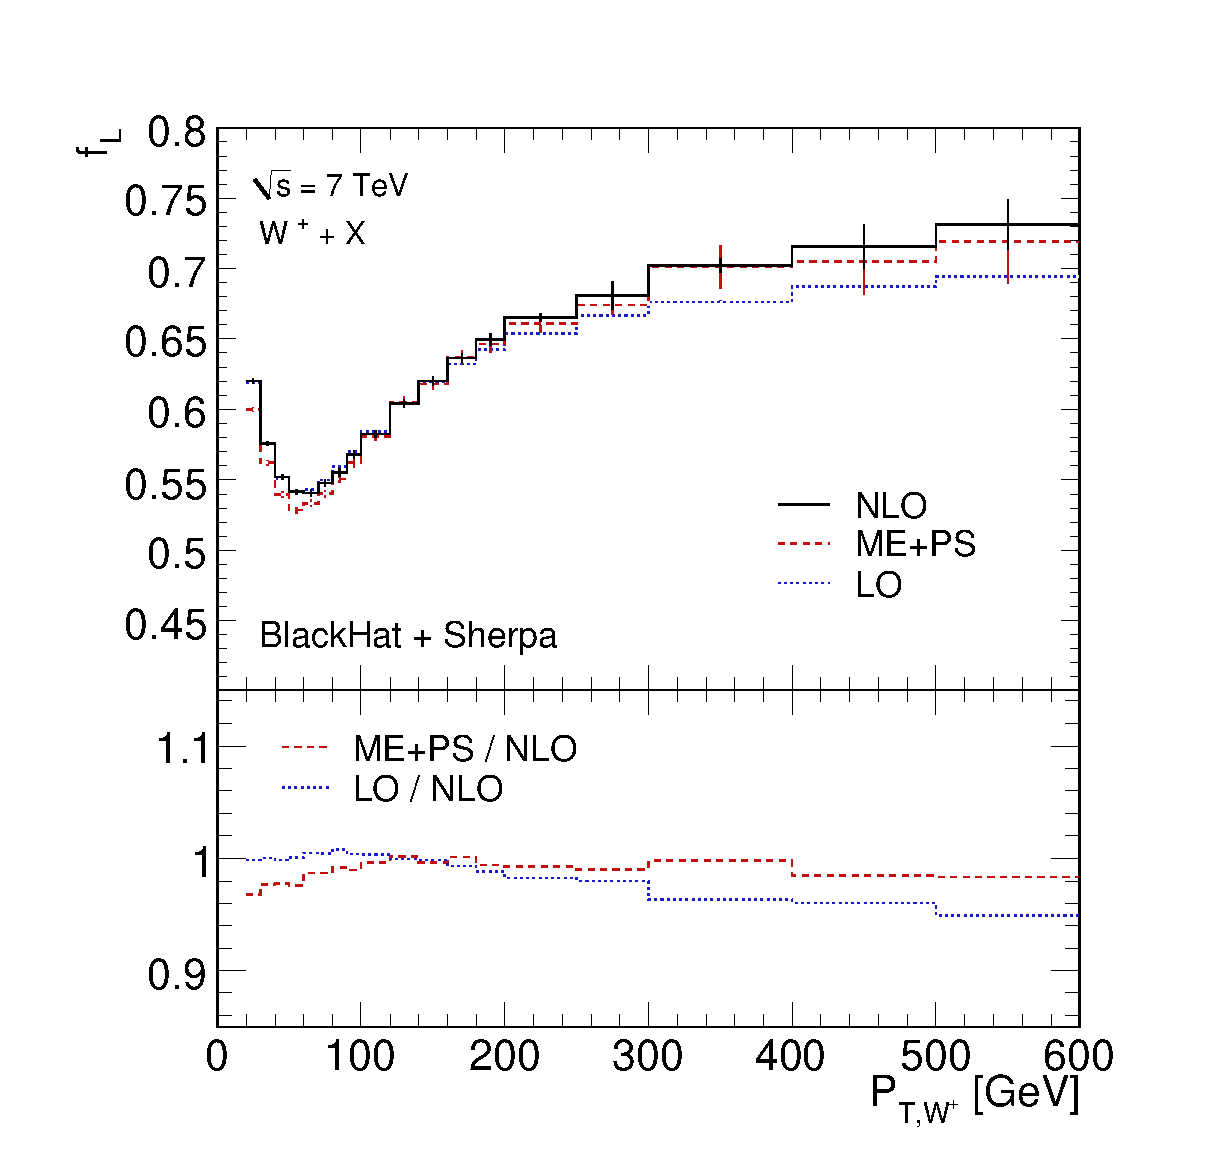
\includegraphics[width=0.32\textwidth]{fig/fL_Wp}}
\subfloat[\fR]{\label{fig:framework_ptw_fR}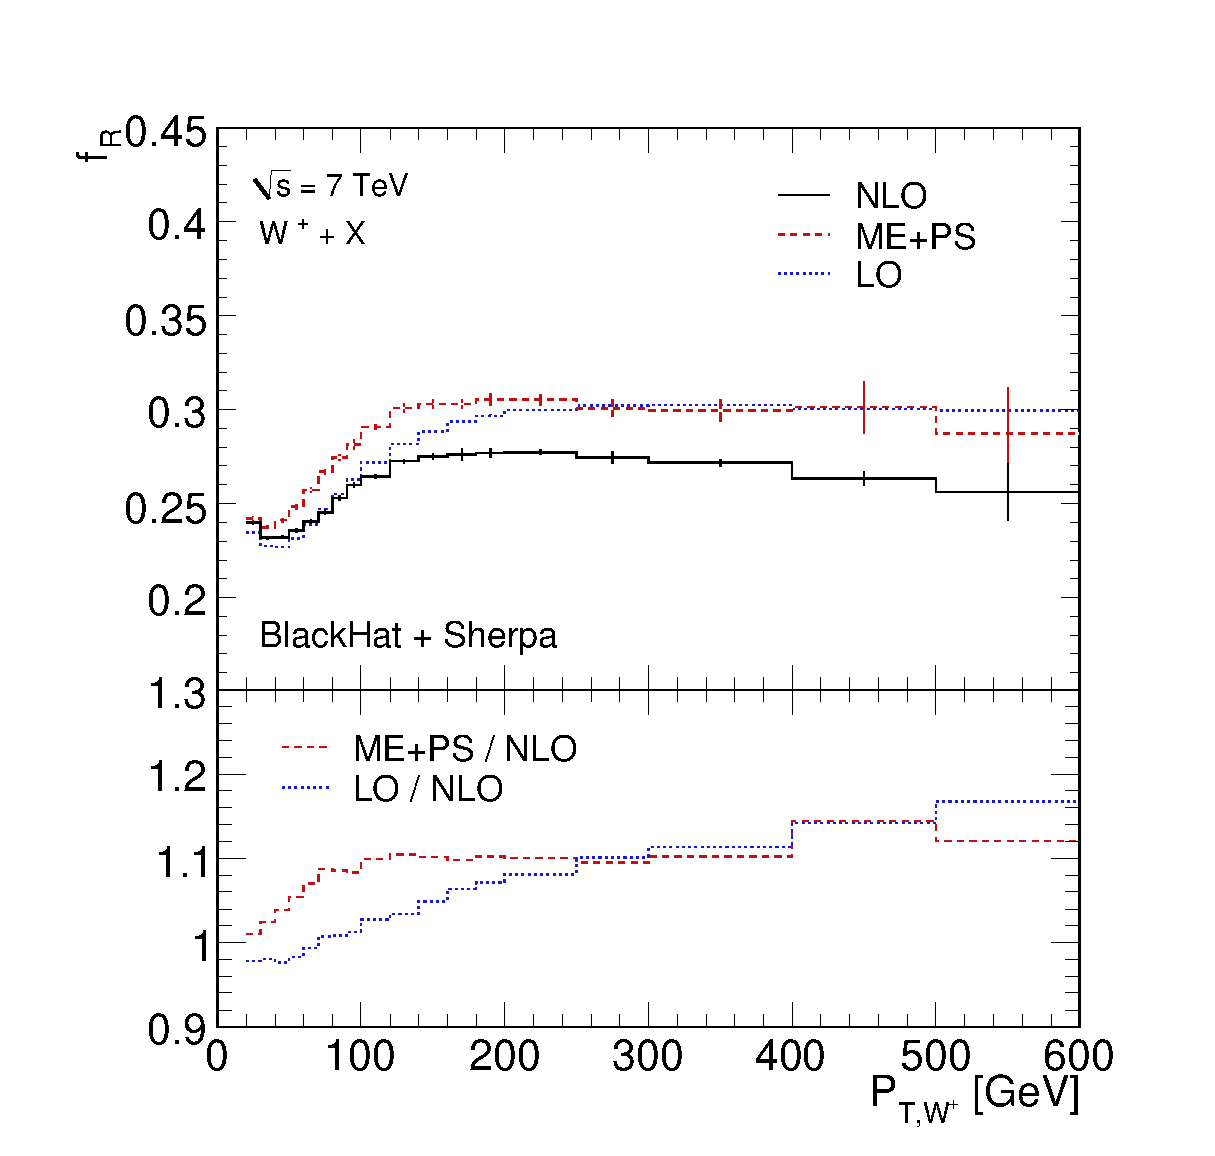
\includegraphics[width=0.32\textwidth]{fig/fR_Wp}}
\subfloat[\f0]{\label{fig:framework_ptw_f0}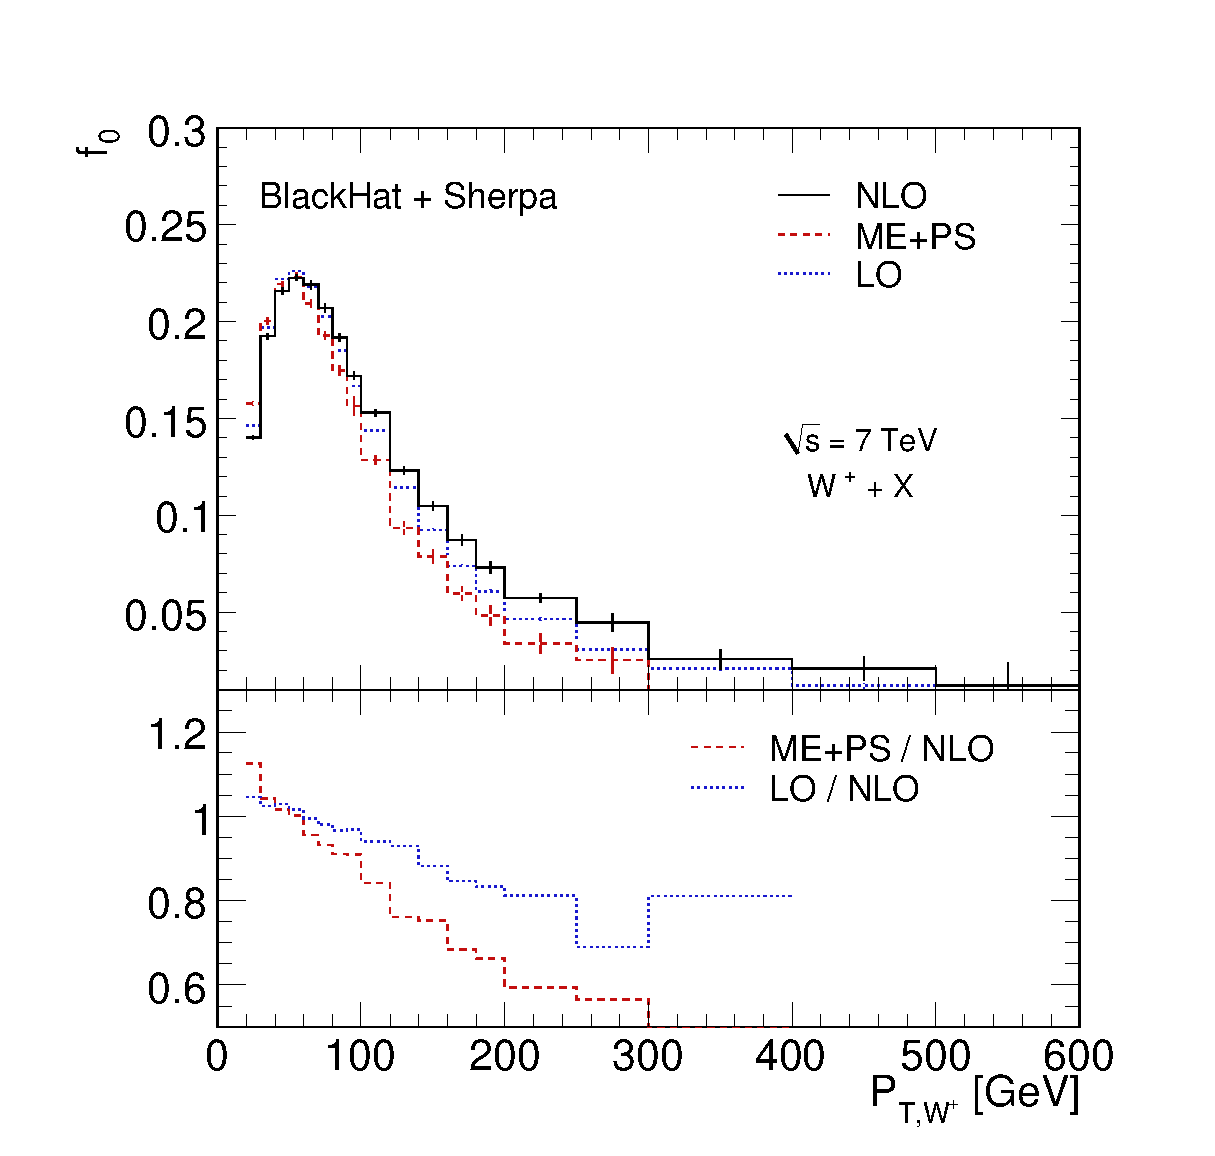
\includegraphics[width=0.32\textwidth]{fig/f0_Wp}}
\caption[The polarisation fractions, \fL, \fR and \f0 as a function of \PtW]{The
  polarisation fractions \fL, \fR and \f0 as a function of \PtW for \PWp
  production are shown in the upper panes of \figs~\ref{fig:framework_ptw_fL},
  \ref{fig:framework_ptw_fR} and \ref{fig:framework_ptw_f0} respectively. Three
  predictions are shown: the fixed-order \ac{NLO} result as a solid black line,
  the \ac{ME+PS} result as red dashed line and the fixed-order \ac{LO} result as
  a dotted blue line. Uncertainties are indicated by thin vertical lines. The
  lower pane in each plot show the ratio of each prediction with respect to the
  \ac{NLO} prediction~\cite{berger_left_handed_w}.}
\label{fig:framework_ptw}
\end{figure}

\section{Modelling New Physics}
\label{sec:framework_susy}
In the following section, a number of models will be presented. All are suitable
for the interpretation of the single lepton \ac{SUSY} search described in
\chap~\ref{sec:susysearch}.

\subsection{The \acl{CMSSM}}
\label{sec:cmssm}
It was said in \chap~\ref{sec:susy} that the \ac{MSSM} is problematic from the
point of view of collider searches due to the extremely large number of
parameters associated with \ac{SUSY} breaking. In order to make quantitative
statements about the sensitivity of a given experimental search, a more
restricted theory must be considered.

One such theory that has often been used is the
\ac{CMSSM}~\cite{sparticles}. The \ac{CMSSM} is inspired by
\ac{mSUGRA}~\cite{kane_minimal}. This proposes a gravity-mediated \ac{SUSY}
breaking mechanism via a hidden sector. This assumption reduces the parameter
space of the \ac{MSSM} to just 5 parameters, 4 of which are continuous:
\begin{itemize}
\item a universal trilinear scalar coupling, $A_0$;
\item a single scalar mass, $m_0$;
\item a single gaugino mass, $m_{\frac{1}{2}}$;
\item $\tan\beta$ where $\beta$ is the ratio of the Higgs' vacuum expectation values and
\item $\textrm{sign}(\mu)$ where $\mu$ is the self-coupling of the Higgs field.
\end{itemize}

Whilst this proves to be a much more practical model from the point of view of
experimental searches, there is no particular reason to assume that \ac{SUSY} is
broken in this way. The restricted parameter space of the \ac{CMSSM} may
disfavour a number of topologies which would appear in a larger class of
\ac{SUSY} theories. One example of this is that the gluino mass parameter, $M_3$
is related to the Bino and Wino mass parameters, $M_1$ and $M_2$ by the
following approximate relation~\cite[p.99]{susy_primer}:
\begin{equation*}
M_3:M_2:M_1 \approx 6:2:1.
\end{equation*}
This relation holds in models with \ac{mSUGRA} or \ac{GMSB} boundary
conditions. However, it is not necessarily the case in more general \ac{SUSY}
theories.

An additional, but related difficulty is that
interpretations of results within the \ac{CMSSM} may not be robustly
extrapolated to alternative models. As will be seen, both of these difficulties
are addressed by a more generic set of \ac{SUSY}-inspired models. These will be
presented in the next section.

\subsection{Simplified Models}
\label{sec:sms}
It is often the case that theorists, having devised some theory, and made
concrete phenomenological predictions from it, wish to test it against
experimental data. The difficulty then arises of taking these predictions and
translating them into a form where they can be compared directly with
experimental results. Typically, these results will be provided in the form of
one or more event yields, corresponding background predictions and statistical
and systematic uncertainties. In some (but probably not most) cases, the
relevant correlations will also be included. The theorist must then take the
predictions of the theory and apply experimental resolution effects to them in
order to simulate the expected signal yield. Modern detectors are highly complex
and require very complex simulation to precisely model all of the resolution and
acceptance effects. In some cases, in particular for relatively simple kinematic
quantities, a simplified parameterisation may suffice. However, detailed checks
will be required to confirm that a given approximation reproduces, with adequate
fidelity the results of the full detector simulation or the actual recorded
data. If it can be confirmed that this is the case, the theorist may then
proceed to redo the work of the experimentalist in modelling the various
statistical and systematic effects in the form of a likelihood
function. Finally, they may then utilise all of these components to produce
their own interpretation of the data against the chosen theory.

Clearly, this procedure is both laborious and error-prone. It was therefore
proposed that the \ac{LHC} experiments would provide a richer interpretation in
the context of a set of \emph{simplified models}~\cite{alwall_simplified}. Broadly
speaking, a simplified model is an effective theory, chosen to characterise a
particular phenomenological scenario present within one or more \ac{NP}
models. Free parameters which have little effect on the physics (at least at
small integrated luminosities) are integrated out, leaving only those with a
greater effect on the physics. By constructing a number of these models, the
full space of possibly physical signatures arising in much more complicated
theories may be spanned. This collection of models is sometimes referred to as a
\acf{SMS}

Although the concept of a simplified model is quite general, the discussion here
will now focus on those inspired by \ac{SUSY} or ``\ac{SUSY}-like'' theories,
and more specifically those giving rise to single lepton final states.

\subsubsection{Dark Matter Models}
As discussed in \chap~\ref{sec:susy}, a highly desirable prediction of certain
supersymmetric theories is the existence of a stable, weakly-interacting
particle or \ac{WIMP}. This is a dark matter candidate with a striking
experimental signature at collider experiments -- a large missing energy
component. Since these topologies are largely inspired by \Rparity conserving
\ac{SUSY}, similar terminology and notation will be used to refer to their
particle content. This should not be taken to suggest that these topologies are
exclusive to \ac{SUSY} type theories.

The topologies considered here may be split into two categories. The first
begins with pair-production of a neutral, coloured object -- the gluino in the
case of \ac{SUSY}. The second is initiated by production of a charged, coloured
object -- the squark of \ac{SUSY} . As for the \ac{CMSSM}, if suitably light,
these are expected to be produced most abundantly at the \ac{LHC}.

In either case, the squark or gluino-type particle then decays, either directly
to an \ac{LSP} or via some intermediate particles (comparable to the heavy
electroweakinos of \ac{SUSY}) -- a cascade decay.
% The naming convention adopted here gives each model a name, T$x$. For models
% resembling pair production of the gluinos, $x$ will be an odd integer and for
% those representing squark production, an even integer. For gluino-type
% topologies, $x$ values of 1, 3 and 5 represent respectively: direct decay of
% both particles, one cascade and one direct decay and two cascade decays. The
% squark-type models are similarly labelled 2, 3 and 4 representing the same
% combinations of direct and cascade decays.

\begin{figure}[htbp!]
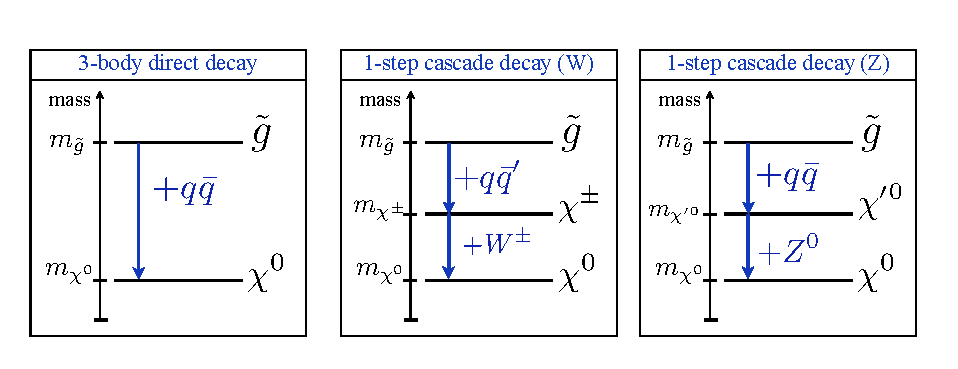
\includegraphics[width=0.8\textwidth]{fig/gluino_sms_decays}
\caption[Illustration of direct and cascade decay modes within simplified
models]{Illustration of direct and cascade gluino decay modes within \ac{SUSY}
  simplified models.~\cite{alves_simplified_2011}}
\label{fig:gluino_sms_decays}
\end{figure}

\subsubsection{Connection to Supersymmetry}
Considering first the gluino pair-production models
(\fig~\ref{fig:gluino_sms_decays}), we shall assume that the squarks are heavier
and therefore kinematically inaccessible. If this were not the case, the
phenomenology would be better described by the squark-type models.

In such supersymmetric models, the gluino may decay only via an off-shell
squark~\cite{alwall_simplified}. This may be either directly to the LSP or
indirectly via intermediate states. Direct decays correspond to \ac{SUSY}
scenarios where either~\cite{alves_simplified_2011}:
\begin{itemize}
\item $\PSgxzi \approx \PSB$ and the $\PSq_{R}$ are lightest or the $\PSW$ is kinematically
  inaccessible;
\item $\PSgxzi \approx \PSW$ and either $\PSq_{L}$ are lightest or there is no
  splitting between the left and right-handed squarks and
\item $\PSgxzi \approx \PSH$ and either heavy-flavour squarks are inaccessible or
  $\PSB$ and $\PSW$ are inaccessible.
\end{itemize}

This is not generally true in either \ac{mSUGRA} or \ac{GMSB} but does
correspond to certain \ac{AMSB} scenarios~\cite{alves_simplified_2011}.

Alternatively, the gluino may undergo a cascade decay via an intermediate mass
state, either a chargino or a heavy neutralino. This will subsequently decay to
the \ac{LSP} via either a $\PW$ or $\PZ$ boson.

The situation is similar in the case of squark pair-production, except that
without the intermediate off-shell squark, the jet multiplicity is
reduced~\cite{alves_simplified_2011}.

\subsubsection{Single Lepton Topologies}
To provide a meaningful interpretation of the single lepton search detailed in
\chap~\ref{sec:susysearch}, two simplified models have been chosen. The models,
\TthreeW and \Ttwott, have been chosen in particular since they offer topologies
which are likely to enter the selection of a single lepton \ac{SUSY} search.

\begin{figure}[htbp!]
\centering
\subfloat[\TthreeW]{\label{fig:sms_topologies_t3w}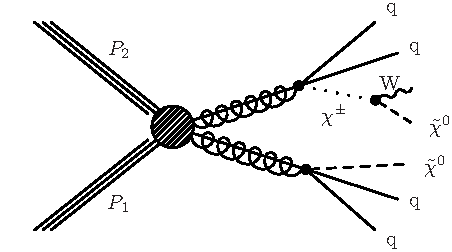
\includegraphics[width=0.45\textwidth]{fig/T3w}}\quad
\subfloat[\Ttwott]{\label{fig:sms_topologies_t2tt}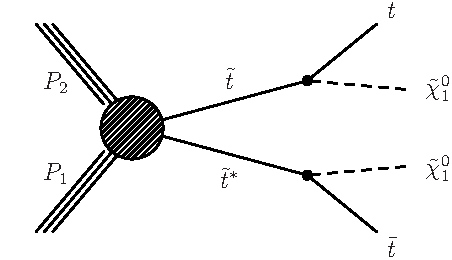
\includegraphics[width=0.45\textwidth]{fig/T2tt}}
\caption[Feynman diagrams illustrating two simplified model topologies]{Feynman
  diagrams illustrating two simplified model topologies suited to a single
  lepton supersymmetry search: \subref{fig:sms_topologies_t3w} \TthreeW and
  \subref{fig:sms_topologies_t2tt} \Ttwott~\cite{susy_interpretation_pas}}
\label{fig:sms_topologies}
\end{figure}

The \TthreeW model is a gluino pair-production model, in which one of the mother
particles undergoes a cascade decay via an intermediate particle. The $\PW$ in
the model name indicates that this intermediate particle is then ``forced'' to
decay to a \PW boson. This topology is illustrated in
\fig~\ref{fig:sms_topologies_t3w} and is seen to be similar to the example
\ac{SUSY} decay illustrated in \fig~\ref{fig:susy_1lep_decay}. This model is
parameterised by the mass of the mother particle, \Mgluino, the mass of the
daughter particle, \Mlsp and the mass of the intermediate particle, \Mchargino.

The second model, \Ttwott, begins with squark pair production. Both mother
particles decay directly to the \ac{LSP}. Furthermore, both squarks are assumed
to be stop particles -- the superpartner of the top quark -- each decaying to a
\ac{SM} top quark. This decay topology is illustrated in
\fig~\ref{fig:sms_topologies_t2tt}. Such events with two top quarks in the final
state, should give an experimental signature suitable for a single lepton
search.

The \Ttwott model reflects scenarios in which the stop is the lightest of the
squarks. These are theoretically attractive for a number of reasons
(see~\cite[{p.~202}]{sparticles} and~\cite{light_stop}). Since this does not
contain an intermediate mass state, it has only two parameters: the mass of the
mother, \Mstop and the mass of the daughter, \Mlsp.

\section{Summary}
A number of theoretical models have been reviewed, each of relevance to the
analysis work presented in \chaps~\ref{sec:wpol}, \ref{sec:susysearch} and
\ref{sec:interpretation}. In the next chapter, aspects of the \ac{CMS}
experiment and the \ac{LHC} will be discussed.
